\chapter{Results}

\minitoc

\newpage

\section{Inter-team Coordination in Large-Scale Globally Distributed Scrum: Do Scrum-of-Scrums Really Work?}

As mentioned in section \ref{scrum} Scrum-of-Scrums (SoS) are considered as the method for handling inter-team coordination in large-scale Scrum projects. In this article by Paasivaara et al. implementation of these so-called SoSs are looked at in a multi-case study of two globally distributed large-scale projects to investigate their success \cite{Paasivaara2012}. The projects were from two different telecom companies. Some information about the projects and data collection is summarised in table \ref{cpadc}.

\begin{table}[H]
\begin{center}
    \begin{tabular}{| p{3.5cm} | p{5.5cm} | p{5.5cm} |}
    \hline
     & \textbf{Case A} & \textbf{Case B} \\ \hline
    Product & Telecommunications, started from scratch & Telecommunications, 10-years old \\ \hline
    Process & Scrum & Incremental change from Waterfall to Scrum  \\ \hline
    Scrum experience & 2,5 years & 1,5 years \\ \hline
    Sites and \# of teams & Finland (10 dev. teams), India (6 dev. teams), Germany (2 test teams), Greece (2 test teams) & Finland (18 teams), Hungary (7 teams) \\ \hline
    Interviews & 19 (Finland 16, Greece 3) & 39 (Finland 28, Hungary 11) \\ \hline
    Roles (The sum exceeds the total number of interviews, as some line managers had double roles, e.g. also worked as Scrum Masters) & Managers (4), Agile coach (1), Scrum Master (1), Developers (5), Testers (2), Line managers (2), Area Product Owners (4), Architects (1) & Managers (6), Agile coach (1), Scrum Masters (6), Team members (13), Line managers (3), Product/Proxy product owners (7), Technical management / architecture (5) \\ \hline
    Interview length & Managers, coach: 1.5-3h, others: 1-1.5h & Managers, coach: 2-3h, others 1-2h \\ \hline
    \end{tabular}
    \caption{Case projects and data collection.}
    \label{cpadc}
\end{center}
\end{table}

\subsection{Findings from Project Cases}
\label{paasivaara}

In Case A the SoS meetings were split into two separate meetings: a Finnish SoS and a Global SoS. The Finnish SoS involved one member from each of the ten development teams located in Finland, as well as the Finnish project manager. In the Global SoS the Finnish project manager led the meetings with one representative from each of the six global development teams and four global test teams present. Initially all questions listed in section \ref{scrum} on Scrum-of-Scrums were answered, but this was later changed because the information gathered from these questions were not perceived as important by all participants. This led to meetings where only impediments or planned impediments for other teams were discussed. Hence, a lot of teams reported to have no problems in their work, which often was not the case, but they felt the other teams did not need to know this information. Managers from Case A confessed that the inter-team communication in the different SoS meetings did not work properly.

In Case B similar issues were faced. Initially the SoS meetings were held only on a global scale, and representatives had problems identifying what to report (as in Case A), and often ended up reporting that there was nothing to share. Because of this a new type of SoS meetings were introduced, namely Feature SoS meetings. In these meetings only teams working on the same features and functionality were present, and all interviewees found the Feature SoSs to be useful. The global SoS meetings were still present, but renamed to Grande SoS meetings. These were still perceived as problematic as attendants found them as uncertain and unnecessary as before.

\subsection{Conclusion}

As can be seen from above it is obvious that the findings show problems with the growing number of participants, especially when these participants have separate interests and concerns. In Case B this was backed up by the success of the smaller Feature SoS meetings focusing on specific functionality. Both case projects also reported a need for project-wide inter-team synchronisation, but had not found any satisfactory solutions.

\section{Communities of Practice in a Large Distributed Agile Software Development Organization – Case Ericsson}

Paasivaara et al. extends the previously discussed study with a deeper analysis of Case B (will be referred to as Ericsson from now on). In the previous study the project consisted of 25 Scrum teams located at two remote sites (Finland and Hungary), this was later expanded. In this case study the Ericsson project involves 40 Scrum teams from the three global sites (Finland, Hungary and the US). The case extends the previous study by looking at a shift from the use of SoS meetings to Community of Practices (CoPs) and will be further outlined below \cite{Paasivaara2014}.

\subsection{Community of Practices Overview}

The CoPs were introduced at the same time as the company made a shift from a traditional software development methodology to an agile approach. Ericsson took use of several different CoPs, the most prominent ones are summarised in table \ref{cop} with their key findings.

\begin{landscape}
\begin{table}
\begin{center}
    \begin{tabular}{| p{3.5cm} | p{4.5cm} | p{4.5cm} | p{4.5cm} | p{4.5cm} |}
    \hline
     & \textbf{Coaching CoP} & \textbf{Feature CoP} & \textbf{Developer CoP} & \textbf{End-to-end CoP} \\ \hline
    Predecessor & Scrum master CoP & SoS and system CoPs & Previous developers' CoP & Program weekly \\ \hline
    Predecessor's role & Sharing experiences in applying Scrum practices & SoS: inter-team coordination, Syst.CoP: feature design & Design rules etc. & High-level R\&D progress monitoring and way of working \\ \hline
    Participants & Scrum masters/coaches & Representatives of cross-functional teams & Developers & Person wanting to make a difference: managers, product owners, coaches, team members \\ \hline
    Current role & Improving the whole organization and its competences & Supporting coordination and design between teams developing a common feature & Software craftsmanship, unifying tools and technologies over product areas & Improve the way of working and optimize the end-to-end flow \\ \hline
    Location and distribution & Cross-site (Finland/Hungary), and site-specific CoPs & According to the distribution of the product areas, mostly cross-site & Finland, Hungary & Finland, Hungary, US \\ \hline
    Rhythm & Weekly & Feature coordination CoPs weekly, Feature design CoPs on a need basis & Bi-weekly & Weekly \\ \hline
    Challenges faced & Lack of common activities and goals after day-to-day problems were solved & Organization-wide SoS did not work: several trials to find a solution to inter-team issues & The first trial ceased to exist due to lack of CoP culture & Involving the US site due to time-zone difference \\ \hline
    Successes & Promising new start with goal to improve the whole organization and its competences & After many trials a functioning solution for inter-team coordination and design & Promising start-up after the death, with a passionate leader, interesting topics and goals & Broad representation of organizational levels and sites facilitates decision making and moving things forward \\ \hline
    \end{tabular}
    \caption{Examples of CoPs at Ericsson.}
    \label{cop}
\end{center}
\end{table}
\end{landscape}

As both the Coaching CoPs and Developer CoPs mainly focus on knowledge sharing these are not further looked into. The interesting CoPs from this study are the Feature CoPs and End-to-end CoPs because of their impact on coordination.

\subsubsection{Feature CoP}

As discussed in section \ref{paasivaara} Feature SoS meetings evolved from the traditional SoS meetings after the troubles with reporting in global SoS meetings. These Feature SoS meetings were held on a weekly basis with approximately 3-8 teams involved in each meeting. Overall there seemed to be a content with these meetings as illustrated in the quotation below from a product owner at the Hungarian site:

\begin{fancyquotes}
Feature SoS meetings are pretty good, because people participating in them work on the same things, talk ‘‘the same language’’ and have a common goal.
\end{fancyquotes}

In parallel with these meetings Ericsson held organization-wide SoS meetings, but these perished. At the same time Feature SoSs were re-branded because of the negative connotations with the word ``SoS''. This led to the introduction of the so-called ``Feature CoPs''. New Feature CoPs were also introduced at the same time, e.g., System CoP.

These Feature SoS/CoP meetings grew further evolving to what was called the ``Feature coordination CoPs'' in the study. These meetings had a timeslot of one hour where about half of that was used at traditional SoS style coordination discussion, and the rest was aimed towards discussing general topics like testing, continuous integration and other improvements. They also witnessed the need to separate the most technical challenges into another meeting which evolved into Feature Design CoP meetings. These seemed to give additional benefits and were seen as well-functioning. As can be seen from the quotation below from one of the developers at the Finnish site, the Feature Design CoPs were self-organising, which is in line with the agile methodologies:

\begin{fancyquotes}
These meetings (Feature Design CoPs) are invited by individuals, it is not Product Owner driven. When somebody feels that we need to do something, he takes the responsibility and invites a meeting. And luckily, there has been interest, and the people that have been needed have participated, and also those that have been interested to learn more have participated. Thus, it is not only the best gurus that discuss together. Instead, it is an open meeting that everybody who wants may participate in. And the invitation is send to everybody. I think it is very important, because if there will be cliques, bad things will happen.
\end{fancyquotes}

\subsubsection{End-to-end CoP}

End-to-end CoPs were introduced to improve the organisation as a whole and to optimise product development flow throughout the whole organisation (removing bottlenecks along the way). The CoP meetings were organisation-wide, even attracting some of the US team members at times. The feedback surrounding the End-to-end CoP meetings had been very good. A quotation from one of the product owners at the Finnish site is included to give an overview of the meetings' contribution:

\begin{fancyquotes}
There, we concentrate on what are the challenges, what we should do to be more efficient as an organization. If we don’t have enough test environments, or certain knowledge, or the way-of-working is bad, or collaboration is not working. From a very broad scale you can bring in topics and there is the head coach and often other managers, people who can easily take things forward.
\end{fancyquotes}

\subsection{Characteristics of Successful CoPs}

From the interviews in the study some characteristics for successful CoPs were extracted. All of them are summarised in figure \ref{CoP}. A few of these will be briefly described: ``Interesting topic and concrete benefits'', ``Open community'' and ``Cross-site participation when needed''.

It is important that CoPs have interesting topics so the participants will feel that they benefit from the meetings. This was especially the case for the Feature CoP meetings where participants had a clear interest in the aspects discussed. For the CoP culture to work it is paramount that the community is open in the sense that they are self-organising. Forced CoPs or meetings that do not interest the participants will not work well. Lastly, it is important that cross-site participation is performed when needed in a globally distributed project. To keep synchronisation and coordination at a high level this is necessary. This was problematic in the initial organisation-wide SoS meetings, but was deemed successful in the End-to-end CoP meetings.

\begin{figure}[H]
\centering
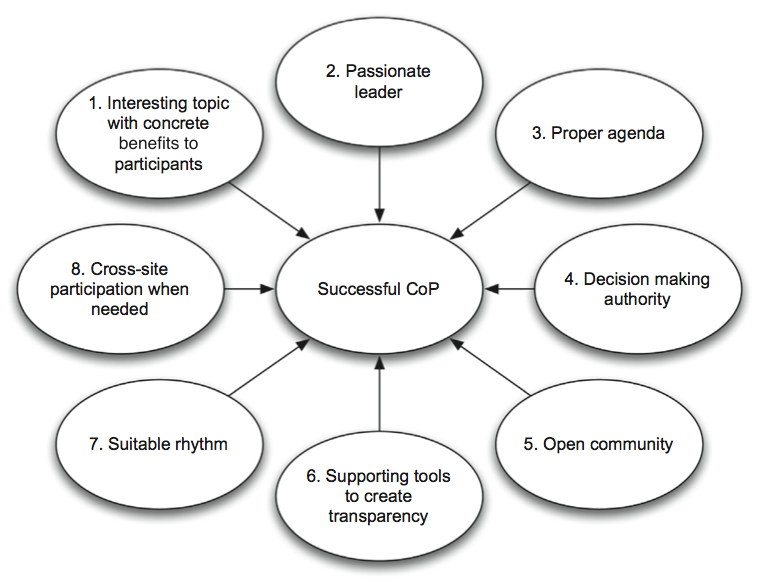
\includegraphics[width=140mm]{images/CoP.png}
\caption{Characteristics of successful CoPs.}
\label{CoP}
\end{figure}

\subsection{Purpose of CoPs}

There were four purposes of the CoPs classified from the study. These are summarised in table \ref{cpae} with an example of each. The focus here will mainly be on the coordination purpose with a quick look at the organisational development.

The aforementioned Feature Coordination CoPs was the main form of inter-team coordination achieved through CoPs. Here several cross-functional teams working on similar functionality or working inside one product area meet and coordinate their work. These types of CoPs were formed when the organisation-wide Scrum-of-Scrum meetings did not deliver expected benefits. In Scrum literature the SoS meetings are seen as a reporting meeting, but here these meetings evolved into discussion meetings focusing on coordination issues, namely the Feature Coordination CoP meetings. The organisational development purpose can indirectly also be seen as a coordination purpose. This has to do with the aim to improve and optimise the product development at an organisation-wide level, which should lead to synchronisation improvements across teams. An example from the study was the End-to-end CoPs.

\begin{table}[H]
\begin{center}
    \begin{tabular}{| p{6cm} | p{6cm} |}
    \hline
    \textbf{Purpose} & \textbf{Example} \\ \hline
    Knowledge sharing and learning & Role-based CoPs \\ \hline
    Coordination & Feature coordination CoP  \\ \hline
    Technical work & System CoPs \\ \hline
    Organisational development & End-to-end CoP \\ \hline
    \end{tabular}
    \caption{CoP purposes at Ericsson.}
    \label{cpae}
\end{center}
\end{table}

\subsection{Findings and Conclusion}

The case study shows how CoPs can be used as a central mechanism for success when introducing a shift from a traditional software development methodology to a large-scale agile approach. CoPs were a central part in knowledge sharing, inter-team coordination and communication, technical work and organisational development. The characteristics for how Ericsson achieved successful CoPs are summarised in figure \ref{CoP}, while table \ref{cpae} illustrates the purpose behind the CoPs. Regarding coordination it is important to note how CoPs gradually replaced the not so successful Scrum-of-Scrum meetings as Ericsson's inter-team coordination method.

Below practical implications are listed for the organisational and management level in the first list, and for the practitioners in the organisation in the second list.

\fbox{\parbox{\textwidth}{Practical implications for the organisational and management level:
\begin{enumerate}
  \item CoPs can support a Lean and Agile transformation. The study suggests that CoPs can be used as an effective mechanism for the transformation from a traditional software development methodology to an agile approach.
  \item CoPs can support scaling agile to a large and distributed organisation. As basic Scrum does not support large-scale cross-team coordination this is an important finding.
  \item Building a CoP-friendly corporate culture is important. For the CoPs to succeed this is crucial aspect.
\end{enumerate}}}

\fbox{\parbox{\textwidth}{Practical implications for the practitioners in the organisation:
\begin{enumerate}
  \item Participate in CoPs and create a new one when needed. CoPs should be self-organising meaning that they are created and disbanded on a need basis.
  \item Use CoPs to learn and further your career. CoPs are a good way of keeping things synchronised, as well as broadening the practitioners knowledge.
  \item Influence the organisation via CoPs. Seeing decisions can be made within CoPs it is important that organisational members attend, and by that influence the direction of the organisation.
\end{enumerate}}}

\section{Towards a Governance Framework for Chains of Scrum Teams}

Vlietland et al. takes a further look at the increasing adoption of agile methodologies in large companies. Their focus is on how the traditional chain of production is handled in the agile approach, or more precisely in Scrum. They aim to identify the collaboration related issues that appear in chains of Scrum teams \cite{Vlietland2015}. Three companies, and their corresponding projects, were investigated and are outlined in table \ref{iacc}. The interviewees consisted of key personnel as Product Owners, line managers and Scrum Master (Scrum Masters were also considered as developers meaning no other Scrum team members were interviewed).

\begin{table}[H]
\begin{center}
    \begin{tabular}{| p{2.25cm} | p{3.75cm} | p{4.5cm} | p{3.75cm} |}
    \hline
     & \textbf{Type of Company} & \textbf{Number of Interviews} & \textbf{Number of Chains} \\ \hline
    Case study 1 & Telecommunications & 9 interviews & Two overlapping chains \\ \hline
    Case study 2 & Insurance & 6 interviews & One chain  \\ \hline
    Case study 3 & Insurance & 3 interviews & One chain \\ \hline
    \end{tabular}
    \caption{Information about case companies.}
    \label{iacc}
\end{center}
\end{table}

\subsection{Issues identified}

From the interview rounds six issue areas were identified. These are outlined in table \ref{gfei}. The distribution of the different issue areas on the three case studies are further showed in table \ref{doiotcs}. What is interesting is that most of these issues directly or indirectly influences coordination, collaboration and/or communication, and are therefore somewhat coupled (this will be easier to understand when looking at the proposed conceptual model in section \ref{conceptualmodel}). The different issue areas are summarised in their corresponding subsections below with suggested propositions. These propositions are summarised in table \ref{sop}.

\begin{table}[ht!]
\begin{center}
    \begin{tabular}{| p{6.5cm} | p{3.75cm} | p{3.75cm} |}
    \hline
    \textbf{Issues description} & \textbf{Issue} & \textbf{Number of quotes} \\ \hline
    A lack of coordination in the chain & Coordination & 124 \\ \hline
    Mismatches in backlog priority between teams & Prioritization & 122 \\ \hline
    Alignment issues between teams & Alignment & 99 \\ \hline
    A lack of IT chain process automation & Automation & 72 \\ \hline
    Unpredictability of delivery to commitment & Predictability & 56 \\ \hline
    A lack of information visibility in the chain & Visibility & 38 \\ \hline
     & Total & 511 \\ \hline
    \end{tabular}
    \caption{Grounding for each issue.}
    \label{gfei}
\end{center}
\end{table}

\begin{table}[ht!]
\begin{center}
    \begin{tabular}{| p{4.5cm} | p{3cm} | p{3cm} | p{3cm} |}
    \hline
    \textbf{Issue} & \textbf{Case 1 (\%)} & \textbf{Case 2 (\%)} & \textbf{Case 3 (\%)} \\ \hline
    Coordination & 29 & 16 & 18 \\ \hline
    Prioritization & 22 & 35 & 17  \\ \hline
    Alignment & 20 & 22 & 13 \\ \hline
    Automation & 14 & 15 & 15 \\ \hline
    Predictability & 11 & 5 & 17 \\ \hline
    Visibility & 4 & 7 & 20 \\ \hline
    Total & 100 & 100 & 100 \\ \hline
    \end{tabular}
    \caption{Distribution of issues over the case studies.}
    \label{doiotcs}
\end{center}
\end{table}

\subsubsection{Predictability}

Predictability has to do with the likelihood that interdependent Scrum team will deliver their feature. If a team does not deliver their feature this will lead to a delay in production. If something is delayed in one sprint it will put more effort on the next sprint introducing major costs from rework, such as retesting and bug fixing, as well as longer time to market.

\subsubsection{Coordination}

Coordination between Scrum teams was identified as the main issue as can be seen in table \ref{gfei}. One of the biggest problems was the focus of the backlog of individual Scrum teams, and not on the end-to-end delivery. This had to do with the perceived lack of influence from management. A problem here is that the Scrum framework supports the coordination theory components on an individual team level, but not for a chain of Scrum teams. Proposition P1 is proposed:

\begin{fancyquotes}
P1: Embedded coordination practices within and between Scrum teams positively impact delivery predictability.
\end{fancyquotes}

\subsubsection{Prioritization}

Priority issues constituted a large portion of the problems encountered in the case studies as well. The main issue in prioritization seems to be mismatching backlog priorities. As each product owner sets his backlog prioritization based on his strategic goals it leads to a mismatch on the front to back chain. This leads to P2:

\begin{fancyquotes}
P2: Matching priority over the front to back chain positively impacts delivery predictability.
\end{fancyquotes}

Further prioritization is a way of goal-setting, but this is a component of coordination theory. Therefore, this has to be matched across all Scrum teams in the chain as a single goal leading to P3:

\begin{fancyquotes}
P3: Matching priority improves front to back coordination practices.
\end{fancyquotes}

The authors also argue that to improve the priority matching over the front to back chain the priority matching has to be done at the strategic level. This implies implementation of strategic decision. Combining bounded rationality theory and decision making strategies proposition four (P4) is suggested:

\begin{fancyquotes}
P4: The implementation of decision making strategies improves matched priority setting.
\end{fancyquotes}

\subsubsection{Alignment}

Misalignment was also identified in the case studies, such as several definitions of done, difference in sprint cycle lengths and misalignment of test activities and test results between Scrum teams. This misalignment muster unpredictability and delays. P5 is proposed:

\begin{fancyquotes}
P5: Alignment between Scrum teams positively impacts delivery predictability.
\end{fancyquotes}

A problem with the Scrum framework is its focus on independent teams. For optimisation, only single teams' processes are looked at. When more teams are introduced a focus has to be shifted towards alignment of work, and how a teams work influences other teams. Using coordination theory again the authors argue that a common shared goal and a coordination mechanism will improve alignment in the chain. This led to P6 and P7:

\begin{fancyquotes}
P6: Matched priority setting positively impacts the alignment between Scrum teams.
\end{fancyquotes}

\begin{fancyquotes}
P7: Coordination practices positively impact the alignment between Scrum teams.
\end{fancyquotes}

\subsubsection{Visibility}

The findings also showed that a lack of visibility disabled teams to take appropriate actions, which could easily lead to uncontrollable impediments later in the sprint. If the codependent teams in the chain have visibility over the backlog they will identify the impediments and can therefore take necessary mitigating actions. Control theory suggests that visibility in the chain will have a positive effect on inter-team coordination. This leads to proposition eight:

\begin{fancyquotes}
P8: Information visibility positively impacts coordination practices.
\end{fancyquotes}

\subsubsection{Automation}

Lastly, we have the sixth identified issue area, namely automation. One recognised issue was the lack of backlog status and progress information of codependent teams. This info should be automated to make mitigating activities possible. Through using supply chain management (SCM) literature Vlietland et al. works out the last proposition for the conceptual model:

\begin{fancyquotes}
P9: Automation of status and progress tracking in the chain positively impacts information visibility.
\end{fancyquotes}

\subsection{Conceptual Model}
\label{conceptualmodel}

Using all the propositions summarised in table \ref{sop} and the six identified issue areas a conceptual model is constructed by the authors. They see the conceptual model as a starting point for the development of a governance framework to mitigate the identified issues in chains of Scrum teams. This conceptual model is illustrated in figure \ref{rcm}.

\begin{figure}[H]
\centering
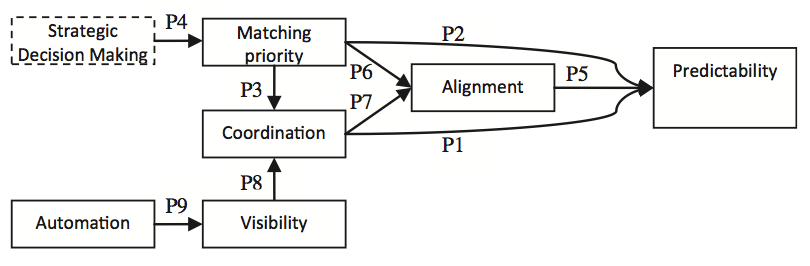
\includegraphics[width=150mm]{images/conceptual_model.png}
\caption{Resulting conceptual model.}
\label{rcm}
\end{figure}

\begin{table}[H]
\begin{center}
    \begin{tabular}{| p{3.25cm} | p{8cm} |}
    \hline
    \textbf{Proposition ID} & \textbf{Proposition} \\ \hline
    P1 & Embedded coordination practices within and between Scrum teams positively impact delivery predictability. \\ \hline
    P2 & Matching priority over the front to back chain positively impacts delivery predictability.
 \\ \hline
    P3 & Matching priority improves front to back coordination practices. \\ \hline
    P4 & The implementation of decision making strategies improves matched priority setting. \\ \hline
    P5 & Alignment between Scrum teams positively impacts delivery predictability. \\ \hline
    P6 & Matched priority setting positively impacts the alignment between Scrum teams. \\ \hline
    P7 & Coordination practices positively impact the alignment between Scrum teams.
 \\ \hline
    P8 & Information visibility positively impacts coordination practices. \\ \hline
    P9 & Automation of status and progress tracking in the chain positively impacts information visibility. \\ \hline
    \end{tabular}
    \caption{Summary of propositions.}
    \label{sop}
\end{center}
\end{table}

\subsection{Conclusion}

Six issues in chains of codependent Scrum teams were identified and are summarised in table \ref{gfei}. From the issue areas and existing theory nine propositions were extracted and are outline in table \ref{sop}. Combining the issues and the propositions the conceptual model in figure \ref{rcm} was created. Coordination is a central part of this puzzle, as can be seen from its direct connection through the propositions to four of the other issue areas (Predictability, Alignment, Visibility and Prioritization/Matching priority), and its indirect connection to the last issue area (Automation) and an added aspect (Strategic Decision Making). It is obvious that the complexity level of coordination is a lot higher in large-scale development, and from Vlietland and Vliet's findings it can be seen that other issue areas need to be addressed together with coordination to achieve a successful and efficient project. It is important to note that this conceptual model needs to be tested in empirical studies to see if it is applicable in practice.